% This is LLNCS.DEM the demonstration file of
% the LaTeX macro package from Springer-Verlag
% for Lecture Notes in Computer Science,
% version 2.4 for LaTeX2e as of 16. April 2010
%
\documentclass{llncs}
%
\usepackage{amsmath}
\usepackage{graphicx}
\usepackage{booktabs}
\usepackage{makeidx}  % allows for indexgeneration
\usepackage{float}
\usepackage{url}
%
\begin{document}
%%
%\frontmatter          % for the preliminaries
%%
%\pagestyle{headings}  % switches on printing of running heads
%\addtocmark{Comparative Analysis of Phonetic Algorithms applied to Spanish} % additional mark in the TOC
%%
%\chapter*{Preface}
%%
%Plan to remove section.
%\vspace{1cm}
%\begin{flushright}\noindent
%July 2016\hfill Axel Garcia\\
%Author\\
%Data Analysis Group UAG
%\end{flushright}
%%
%\chapter*{Organization}
%Plan to remove section.
%%
%\section*{Section Title}
%\begin{tabular}{@{}p{5cm}@{}p{7.2cm}@{}}
%<Role>:&Name
%\end{tabular}
%%
%\begin{multicols}{3}[\section*{Referees}]
%Name 1\\
%Name 2\\
%Name 3
%\end{multicols}
%%
%\section*{Sponsoring Institutions}
%%
%Plan to remove section.
%%
%\tableofcontents
%
\mainmatter              % start of the contributions
%
\title{Comparative Analysis of Phonetic Algorithms Applied to Spanish}
%
\titlerunning{Comparative Analysis}  % abbreviated title (for running head)
%                                     also used for the TOC unless
%                                     \toctitle is used
%
\author{Axel A. Garcia Fuentes\and Rogelio Davila}
%
\authorrunning{Axel A. Garcia Fuentes et al.} % abbreviated author list (for running head)
%
%%%% list of authors for the TOC (use if author list has to be modified)
\tocauthor{Axel A. Garcia Fuentes, and Rogelio Davila}
%
\institute{Universidad Autonoma de Guadalajara, Guadalajara, Mexico,\\
\email{axel.garcia@edu.uag.mx, rogelio.davila@edu.uag.mx}}

\maketitle              % typeset the title of the contribution

\begin{abstract}
Natural language writing is a field of interest. Part of this process is related to 
the written language. Something that is true about that is you can make mistakes 
when writing or typing. Typographical errors are an example of those mistakes. 
Those errors may be imperceptible to a human being, but still, harmless as they 
may seem they may be sufficient to cause a failure when searching a record in 
a database . Could a phonetic algorithm capture enough of the word sound 
essence as to be considered a meaningful resource for colloquial Spanish?\dots
\keywords{Natural Language Processing, Spanish, Phonetic algorithm}
\end{abstract}
%
\section{Introduction}
%
Recently in history there have been efforts on finding an algorithm capable
% Add reference to the census of 1930 in US.
of encode the sound of a word. A the beginning of the 20th century in USA 
those efforts were a resource during the people census in that country.
Names of several places in the world had to be inputted and several of them
did not have a clear writing for the data analysts. That typographic error most
likely is being caused by the homophony between several names. That is
called homonym\cite{ref:14}. Whereas Smith and Schmit sound very similar 
to people, certainly they are not the same for a database computer system. 
Something had to be done in order to properly classify or to correctly index 
the names of all those people.\\

One of the first algorithms used for this purpose is Soundex. It was used for
a while until it was realized it was not helping enough for foreign names. Then
some variants were used: e.g.: Russell Soundex, Daitch-Mokotoff Soundex to
mention a couple of them. More phonetic algorithms were created later, e.g.: 
NYIIS, Metaphone, Beider-Morse Phonetic Matching, Koelner Phonetik, MRA,
and PhoneticSpanish to mention some of them.\\

Objective of those algorithms is to create a resulting code that represents
the sound that a given word may produce when it is pronounced. That means, 
for any arbitrary pair of words, if they share the same resulting code then they are
homophones, i.e. they are pronounced exactly in the same way. The combination of 
the characters (letters) in the word will create the word sound when it is pronounced. 
In a similar way, the algorithm uses the letters that compose the word as input. Trying 
to mimic the effect they have in the word sound, it will use those letters interactions 
in order to create a sound code which will be referred as phonetic code. \\

Something to have in mind also is, even if we can find homophones that does not imply
they are homonyms. The fact that words sound the same is not enough to cause the
words to share the same meaning. There is a deep difference between sound and 
meaning. However, as scope definition of the discussed algorithms, for now the focus is
the sound of the word. This document will disregard its meaning. \\

When we hear the sound of a word when it is pronounced we can remember its 
meaning inside our head. Maybe in the future computers could use the phonetic code 
for natural language processing, too. However, before getting to that stage it is
necessary to chose the algorithm that best describe the sound of a word and as the
document will discuss, that depends on the language. This time the discussion is
about Spanish language, so that will be used for measurements and conclusions. 
Another, aspect to consider is the communication channel. There is oral communication 
and written communication. This discussion elaborates on the later leaving out the former.
The question to answer is, what algorithm is the most convenient to model the sound 
of a word pronounced in Spanish?
 
\section{Phonetic Algorithms}
The variety of names given to the discussed algorithms so far considers: name encoding algorithms\cite{ref:17}, 
phonetic algorithms\cite{ref:01} and phonetic coding algorithms\cite{ref:10}, 
to mention some of them. The former refers to the usage these algorithms have had in recent 
history, notwithstanding, that name suggests those are encoding algorithms. Since what those 
algorithms do is tightly related to the pronunciation of the words, that name may be leaving out
part of those algorithms essence. Last two names mention the concept of "phonetics". In linguistics 
there exist two major areas that study the sound of the words: i.e. phonetics and phonology. Both 
areas have different purposes. Understanding that is recommended to continue the discussion
about these algorithms.

\subsection{Phonetic and Phonology}
% Revise linguistic terms: aparato fonador, a lengua, la garganta, las cuerdas vocales, el paladar, el velo del paladar, los alv�olos, los dientes y los labios
As previously mentioned these algorithms should generate different phonetic codes depending 
on the sound of the word they are processing. Nevertheless, what exactly these algorithms are
processing?. To answer that question it is necessary to talk a little bit about linguistics. That
science has a couple of branches that study the sound of the words. They are phonetics and
phonology\cite{ref:03}. Phonetics study the way in which pronunciation sounds are generated.
For that purpose it uses acoustic analyses, as well as, analyses of what sounds are heard by the
human ear. It elaborates more on the way people articulates the sounds. It considers in those 
analyses the parts of the phonic apparatus: tongue, throat, vocal cords, palate, soft palate, 
alveolus, teeth and lips\cite{ref:06}\cite{ref:07}\cite{ref:18}.\\

Phonology is a complement. That knowledge area studies how the sounds affect the language.
It studies the invariant significant elements of the words. For example, in the word "dedo" (i.e. 
finger in English) each one of the two letters "d" produce a slightly different sound. If that sound
were switched, i.e. pronounce the second "d" as the first one and vice versa, the word would 
sound different (like incorrectly pronounced) but even so it would still be understood as the same
word. As another example, if the second letter "d" were changed to letter "j", then the word would be
"dejo" ("I leave" in English) and the meaning of the word would be different. That last is an example
of a sound that should be invariant in the word "dedo"\cite{ref:04}\cite{ref:05}. Linguistics call 
"phonemes" to those sounds that should be invariant in order to keep the word meaning. 
Phonology studies phonemes (among other language aspects). Phonemes vary in each language, 
i.e. there are different phonemes in English than there are phonemes in Spanish, which in turn are 
different to German, Japanese, and so on. Thus phonemes are language dependent\cite{ref:06}\cite{ref:07}\cite{ref:18}.\\

Phonemes may be considered the functional reference to compare the sound of two words. If there is a 
difference in the phonemes used, then there are two different words being 
compared and the ideal algorithm should produce different resulting codes. Thus what the
algorithm is doing is processing the word in a phonological level. That may be enough 
justification to name these algorithms "phonological algorithms" and to refer to their result
"phonological code". However,  since the name "phonetic algorithms" seems to have been 
widely used by now, this document will use "phonetic algorithms" and "phonetic codes" for 
the rest of the discussion. 

\subsection{Phonetic Algorithms as Hash Algorithms}
Something to have in mind is phonetic algorithms were originally created to index words by the sound 
they produce when pronounced\cite{ref:02}. Using that as base, (in Spanish) "coro" and "koro" should
share the same phonetic code, whereas, "coro" and "choro" should not.  \\

Phonetic codes have been referred to as "phonetic hash". There is a number of desirable 
characteristics that a hash function should meet\cite{ref:16}. Phonetic algorithms are in deed hash 
functions and the reasoning is the following:
\begin{description}
\item[Weak Collision Resistance.] For any given word, if its pronunciation significantly changes then the 
phonetic algorithm should generate a different phonetic code.
\item[Strong Collision Resistance.] Consider those algorithms have been designed to generate the same
phonetic code for words that share the same pronunciation. In that way words can be grouped by phonetic
code. Two words that sound different should have different phonetic codes. That means phonetic 
algorithms are designed for low collision.
\item[Oneway Property.] Phonetic algorithms will ignore characters that are irrelevant to phonetic code 
production. It is not possible to turn it into the initial word since there is not enough information in the 
phonetic code to do it.
\item[Performance.] Phonetic algorithms are deterministic. Some of them look the characters of the word
in a map/dictionary that contains the phonetic code transformation. Structures like maps or dictionaries use
to be O(n) where n is equals to the word length or less. Assuming that a word has a small number of 
characters, then their computation time is reasonable.
\end{description}


There are some phonetic algorithms that has been created. Some of them were designed to process text 
assuming an English context. Some others where extended to languages other than English. Next 
sections will discuss some of the phonetic algorithms that has been used in the past.
 
\subsection{Soundex}
It was used in 1930 during retrospective analysis of US census of 1890-1920\cite{ref:01}. It was used to 
index given names based on their pronunciation in English. Each Soundex code consist of a letter and
three digits; e.g. W�252. The letter us the initial of the surname. The digits are assigned based on the 
subsequent letters in the surname. The objective is to build a code of four elements; zeros are padded
as required\cite{ref:02}\cite{ref:24}.


\subsection{NYSIIS (New York State Identification and Intelligence System)}
Developed circa 1970 after several attempts to improve the Soundex algorithm. NYSIIS creates a 
string of up to six characters. See more details in \cite{ref:17}\cite{ref:24}.


\subsection{Daitch-Mokotoff Soundex System}
Created by Ranndy Daitch and Gary Mokotoff from Jewish Genealogical Society. in 1985 Mokotoff 
indexed the names of 28,000 people that legally changed their names while living in Palestine during 
1921 through 1948. The majority of them were Jewish with germanic or slavic names. During that
exercise there were names that sounded the same. However, Soundex did not generate the same
phonetic code; e.g. Moskowitz y Moskovitz\cite{ref:08}\cite{ref:02}\cite{ref:24}.


\subsection{Metaphone}
It was published in 1990 as an enhancement to Soundex. It was designed for English language.
This phonetic algorithm has been used to perform genealogical searches. There are versions of
this algorithm implemented for high level languages like: Pythoh and PHP to mention some\cite{ref:11}
\cite{ref:12}\cite{ref:13}\cite{ref:22}\cite{ref:24}


\subsection{Double-Metaphone}
It was developed circa 2000. It is an improvement to Metaphone. It produces two phonetic codes 
for a single input word. The two phonetic codes are: the most likely pronunciation and the optimum 
pronunciation\cite{ref:17}\cite{ref:24}.


\subsection{Beider-Morse Phonetic Matching}
This algorithm considers that the pronunciation of a given word depends on the language
where that word is being pronounced. First step is to identify the word language. Then
the word is analyzed and broken down into phonetic tokens. That is performed by using
pronunciation rules for the detected language. Phonetic code is the sequence of phonetic
codes\cite{ref:19}\cite{ref:24}.


\subsection{PhoneticSpanish}
This is a an algorithm proposed by\cite{ref:09} which is based on Soundex. The algorithm
tries to adapt Soundex to Spanish pronunciation. Authors does not mention any restriction
on the phonetic code length.

\section{Phonetic Algorithms Comparison Method}
\subsection{Precision Function}
\label{sec:PrecisionFunction} 
This section explains the shape of the mathematical function used to measure the studied
phonetic algorithm. \\

Each phonetic algorithm generates a phonetic code for a given word: $\phi(\alpha)=\alpha'$
It is possible that a a word could be associated to a distinct phonetic code depending on
the used phonetic algorithm:
\begin{equation}
% ??. ?1(?)=?1? , ?2(?)=?2? , ?3(?)=?3? ? ?1? =/ ?2? =/ ?3?
\exists\alpha.\ \ \phi_1(\alpha)=\alpha'_1,\phi_2(\alpha)=\alpha'_2,\phi_3(\alpha)=\alpha'_3\ \ \land\ \alpha'_1\ne\alpha'_2,\alpha'_2\ne\alpha'_3,\alpha'_3\ne\alpha'_1,
\end{equation}

One of the goals of this comparison is to gather data that allows measure how the studied
phonetic algorithms point to the correct word. In other words, how precise and accurate each
algorithm is. 
\begin{description}
\item[Algorithm Accuracy.] Lets assume there are two words: correct word and a single evaluation word. If 
we were to process evaluation word to find the correct word, then that processing is one step away
from the result; i.e. processing evaluation word will give as result the correct word. If we had two
evaluation words the processing would be two steps away, in the worst case. If there were three evaluation words
then the evaluation would be three steps away, and so on. Precision is how far the processing is
from the correct word. Which in few words mean, how many words share the same phonetic 
code given a phonetic algorithm. Paragraphs below explain that with more details.
\item[Algorithm Precision.] The evaluation word phonetic code matches the correct 
word phonetic code.
\end{description}

The name used in this document for the set of words that share the same phonetic code is 
"recommendation set". Each one of those words are considered a valid replacement alternative. 
Consider the following premises:
\begin{enumerate}
% 1
\item Based on the discussion about phonetics, the pronunciation of each one of the alternatives $\beta$
is equal to the pronunciation of the evaluation word $\alpha$. Thus, assumption is either of those $\beta$
could replace $\alpha$:
\begin{equation}
%????. p(?) = p(?) ? ? ? ?, ???????
\forall\alpha.\beta.\Theta.\left\{\ (p(\alpha) = p(\beta)) \to \alpha=\beta,\ \ \beta\in\Theta\right\}
\end{equation}

% 2
\item However, only a single one of them can be part of the solution set $\Psi$. The rest of them are considered
false positives (FP):
\begin{equation}
\label{eq_01}
%????. ??? ???? ? |?| = 1
\forall\beta.\gamma.\Theta.\Psi.\ (\beta\in\Theta\land\gamma\in\Theta)\land \gamma\ne\beta \to(\gamma\in\Psi\ \land\ \beta\notin\Psi\ \land\ \left\|\Psi\right\|=1)
\end{equation}

% 3
\item A False Negative (FN) is actually a True Positive (TP) incorrectly classified. Based on \ref{eq_01}, true positives set $\Psi$ has a single element $\gamma$. Thus, in this context FN and TP are considered the same:
\begin{equation}
%??. ~~ ? ? ?
\forall\gamma.\Psi.((\neg\neg\gamma\in\Psi\land\gamma\in\Psi\land\left\|\Psi\right\|=1)\to\neg\neg\gamma=\gamma)
\end{equation}
\begin{equation}
TP+FN=1
\end{equation}

% 4
\item Phonetic codes are True Positives candidates. As \ref{eq_01} states there is a single one 
TP, the other $\beta$ candidates are a False Positives(FP), and they are represented by 
$\Delta$ set:
\begin{equation}
\label{eq_02}
\forall\beta.\gamma.\Delta.\ (\beta\in\Delta\land\gamma\notin\Delta) \to\left\|\Delta\right\|=N-1
\end{equation}
Where $N$ is the length of the alternatives set $\Theta$.
\begin{equation}
\left\|\Theta\right\|=N
\end{equation}

% 5
\item 
By definition phonetic codes are TP candidates. That means none of them is meant not to be
an alternative candidate and thus none of them is a True Negative(TN)
\begin{equation}
TN=0
\end{equation}

% 6
\item Accuracy equation has the following form:
\begin{equation}
accuracy=\frac{TP+ TN}{TP + FP + FN + TN}
\label{eq_03}
\end{equation}

Updating \ref{eq_03} with considerations of \ref{eq_01} and \ref{eq_02} precision equation has the following transformation:
\begin{equation}
accuracy=\frac{TP+ TN}{(TP + FN) + (TN+ FP)} \to \frac{TP+ 0}{1 + (N-1)} \to \frac{TP}{N}
\label{eq_05}
\end{equation}


% 7
\item Precision equation has the following form:
\begin{equation}
precision=\frac{TP}{TP + FP}
\label{eq_04}
\end{equation}

Updating \ref{eq_04} with considerations of \ref{eq_01} and \ref{eq_02} precision equation has the following transformation:
\begin{equation}
precision=\frac{TP}{TP + FP} \to \frac{TP}{1 + (N-1)} \to \frac{TP}{N}
\label{eq_06}
\end{equation}


\end{enumerate}

From equations \ref{eq_05} and \ref{eq_06} precision and accuracy are measured 
in the same way. Thus, the function used for this
\[   
precision = 
     \begin{cases}
       \text{$\frac{1}{N}$}\quad\text{Correct word found}\\
       \text{$0$}\quad\text{Otherwise}\
     \end{cases}
\]


\section{Method}
A sample of 1000 tweets was used for this experiment. Those tweets were gathered
without a particular constrain. The text in those tweets is natural language in Spanish
spoken in Mexico. That includes slang, words created by the tweet author, text 
emoticons, as well as, official Spanish words. The input data also has structured strings 
like: urls, numbers and hashtags to mention some.\\

A Python script was used for this evaluation. That evaluation script uses a non-standard 
dictionary of terms. That Spanish dictionary of terms gathers words written in Spanish
which were collected from several public resources. That made it useful for this work.
Evaluation is divided in the following stages:

\begin{description}
\item[Phonetic Code Generation.] Dictionary of terms was processed with each one of
the discussed algorithms. That generated a phonetic code for each one of the terms in
the dictionary. Phonetic codes were added into the dictionary of terms. The result is
the phonetic codes dictionary. \\

\item[Precision Data Generation.] For each one of the sample tweets, each one of the 
words in the tweet was searched in the dictionary of terms. Some words were found 
and some were not. The not found words were processed with the phonetic algorithm.
Their phonetic code was computed, associated to the not-found term and stored in a
different data resource for later use. That means, only the not-found terms were used
for the phonetic algorithm precision measurement. It was decided that way in order to
have a meaningful comparison; since terms found in the dictionary of terms are 
correctly formed by definition.\\

Data generated by this processing was saved in a comma-separated values file (cvs).
Each row in that file has the data generated by the processing done for a single word.
In other words, if a single tweet has several not-found words then there will be multiple
rows for that single tweet. The output CSV file is referred to as output map.\\

\item[Results Generation.] Comparison function mentioned in section \ref{sec:PrecisionFunction} 
was used in this stage. 

\end{description}

Algorithms execution time was not considered. Focus is the precision and accuracy of
the studied phonetic algorithms.

\subsection{Comparison Risks}
Used Spanish dictionary of terms has a mixture of official and non-official Spanish words, 
meaning the Royal Spanish Academy(Spanish: Real Academia Espa\~nola) does not 
recognize some of them. However, that is considered a positive aspect for this 
experiment because in the case of a misspelling that kind of words(non-official) are
most likely to occur in natural language processing. Nevertheless, risk of a bias in the
manual labeling exist. That risk is mitigated with a big sample size and re-using labeled
dictionary for all of the phonetic algorithms evaluations.


\section{Results}
Table \ref{tab:01} shows the studied phonetic algorithms ascendantly ordered by mean
as first criteria and then by variance. That is, the lower in the table the algorithm is the
better precision it has.

\begin{table}[H]
\caption{Phonetic Algorithms: Descriptive Statistics} \label{tab:01}
%\begin{center}
\centering
\begin{tabular}{ lccccc }\\
\toprule[1.5pt]
	\bf Algorithm & \bf Mean & \bf Mode & \bf Median & \bf Variance & \bf Std Dev \\ \hline
         Phonex	&0.0010&	-	&0.0008	&0.0000	&0.0006\\
         Fuzzy Soundex	&0.0081	&-	&0.0058	&0.0000	&0.0071\\
         Rusell Index	&0.0164	&-	&0.0115	&0.0002	&0.0140\\
         Phonix	&0.0169	&-	&0.0129	&0.0002	&0.0129\\
         Alpha Sis	&0.0191	&-	&0.0143	&0.0003	&0.0161\\
         Soundex	&0.0202	&-	&0.0165	&0.0002	&0.0137\\
         Double Metaphone	&0.0224	&-	&0.0178	&0.0003	&0.0179\\
         Phonetik	&0.0253	&-	&0.0183	&0.0004	&0.0207\\
         Sfinixbis	&0.0278	&0.0243	&0.0243	&0.0003	&0.0165\\
         Caverphone	&0.0317	&-	&0.0252	&0.0006	&0.0235\\
         MRA	&0.0416	&0.0000	&0.0374	&0.0006	&0.0243\\
         Metaphone	&0.0464	&-	&0.0416	&0.0008	&0.0287\\
         BMPM	&0.0532	&-	&0.0497	&0.0009	&0.0302\\
         NYSIIS	&0.0536	&-	&0.0474	&0.0010	&0.0318\\
         Phonet	&0.0838	&-	&0.0803	&0.0013	&0.0355\\
         Phonem	&0.1036	&-	&0.1011	&0.0020	&0.0444\\
\bottomrule[1.25pt]
\end{tabular}
%\end{center}
\label{default}
\end{table}%


\begin{figure}
\begin{center}
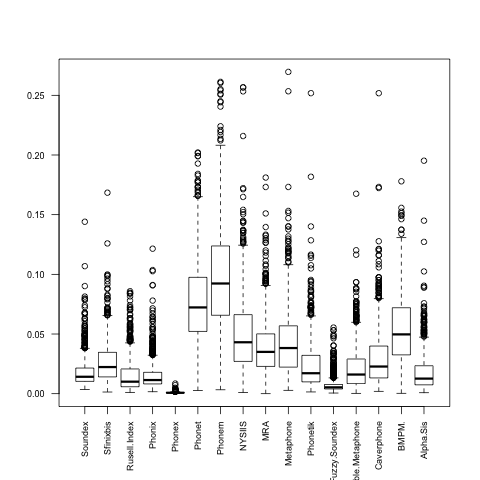
\includegraphics[width=0.9\textwidth, height=10cm]{images/boxplot.png}
\caption{default}
\label{default}
\end{center}
\end{figure}


\section{Conclusions}
Phonem and Phonet are the two algorithms with the best descriptive statistics
since they have the highest precision mean. Phonet has lower variability than
Phonem and the variance-precision ratio is better for Phonet also. That fact
suggests Phonet may give better results for natural language processing applied
to Spanish texts.

%
% ---- Bibliography ----
%

\bibliographystyle{ieeetr}
\bibliography{biblio}



\clearpage
\addtocmark[2]{Author Index} % additional numbered TOC entry
\renewcommand{\indexname}{Author Index}
\printindex
\clearpage

\end{document}
